\let\negmedspace\undefined
\let\negthickspace\undefined
\documentclass[journal]{IEEEtran}
\usepackage[a5paper, margin=10mm, onecolumn]{geometry}
%\usepackage{lmodern} % Ensure lmodern is loaded for pdflatex
\usepackage{tfrupee} % Include tfrupee package

\setlength{\headheight}{1cm} % Set the height of the header box
\setlength{\headsep}{0mm}  % Set the distance between the header box and the top of the text

\usepackage{gvv-book}
\usepackage{gvv}
\usepackage{cite}
\usepackage{amsmath,amssymb,amsfonts,amsthm}
\usepackage{algorithmic}
\usepackage{graphicx}
\usepackage{textcomp}
\usepackage{xcolor}
\usepackage{txfonts}
\usepackage{listings}
\usepackage{enumitem}
\usepackage{mathtools}
\usepackage{gensymb}
\usepackage{comment}
\usepackage[breaklinks=true]{hyperref}
\usepackage{tkz-euclide} 
\usepackage{listings}
% \usepackage{gvv}                                        
\def\inputGnumericTable{}                      
           
\usepackage[latin1]{inputenc}                                
\usepackage{color}                                            
\usepackage{array}             
                               
\usepackage{longtable}                                       
\usepackage{calc}
\usepackage{caption}
\usepackage{multirow}                              
           
\usepackage{hhline}                                           
\usepackage{ifthen}                                           
\usepackage{lscape}
\usepackage{tikz}
\usetikzlibrary{patterns}

\title{\textbf{GATE 2025 ES}}
\author{ee25btech11035 - Kushal B N}
\begin{document}
\maketitle
\section*{General Aptitude}

\subsection*{Q.1 -- Q.5 Carry ONE mark Each}

\begin{enumerate}
\item Courage: Bravery :: Yearning : \_\_\_\_\_\_\_\_ \\
Select the most appropriate option to complete the analogy.
\hfill{\brak{GATE~ES~2025}}
\begin{enumerate}
\item Longing
\item Yelling
\item Yawning
\item Glaring
\end{enumerate}

\item We \_\_\_\_\_\_\_\_\_\_\_\_\_\_ tennis in the lawn when it suddenly started to rain. \\
Select the most appropriate option to complete the above sentence.
\hfill{\brak{GATE~ES~2025}}
\begin{enumerate}
\item have been playing
\item had been playing
\item would have been playing
\item could be playing
\end{enumerate}

\item A $4 \times 4$ digital image has pixel intensities ($U$) as shown in the figure. The number of pixels with $U \le 4$ is:
\hfill{\brak{GATE~ES~2025}}
\begin{center}
\begin{tabular}{|c|c|c|c|}
\hline
0 & 1 & 0 & 2 \\
\hline
4 & 7 & 3 & 3 \\
\hline
5 & 5 & 4 & 4 \\
\hline
6 & 7 & 3 & 2 \\
\hline
\end{tabular}
\end{center}
\begin{enumerate}
\item 3
\item 8
\item 11
\item 9
\end{enumerate}

\item In the given \figref{fig1}, the numbers associated with the rectangle, triangle, and ellipse are 1, 2, and 3, respectively. Which one among the given options is the most appropriate combination of $P$, $Q$, and $R$?
\begin{figure}[H]
    \centering
    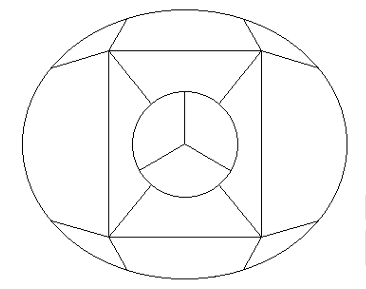
\includegraphics[width=0.4\columnwidth]{figs/fig1.png}
    \caption{Figure for Q.4}
    \label{fig1}
\end{figure}
\hfill{\brak{GATE~ES~2025}}
\begin{enumerate}
\item $P$ = 6; $Q$ = 5; $R$ = 3
\item $P$ = 5; $Q$ = 6; $R$ = 3
\item $P$ = 3; $Q$ = 6; $R$ = 6
\item $P$ = 5; $Q$ = 3; $R$ = 6
\end{enumerate}

\item A rectangle has a length $L$ and a width $W$, where $L > W$. If the width, $W$, is increased by 10\%, which one of the following statements is correct for all values of $L$ and $W$?
\hfill{\brak{GATE~ES~2025}}
\begin{enumerate}
\item Perimeter increases by 10\%.
\item Length of the diagonals increases by 10\%.
\item Area increases by 10\%.
\item The rectangle becomes a square.
\end{enumerate}

\subsection*{Q.6 -- Q.10 Carry TWO marks Each}

\item Column-I has statements made by Shanthala; and, Column-II has responses given by Kanishk.
\begin{center}
\begin{tabular}{|l|p{5cm}|l|p{5cm}|}
\hline
\multicolumn{2}{|c|}{\textbf{Column-I}} & \multicolumn{2}{c|}{\textbf{Column-II}} \\
\hline
P. & This house is in a mess. & 1. & Alright, I won't bring it up during our conversations. \\
\hline
Q. & I am not happy with the marks given to me. & 2. & Well, you can easily look it up. \\
\hline
R. & Politics is a subject I avoid talking about. & 3. & No problem, let me clear it up for you. \\
\hline
S. & I don't know what this word means. & 4. & Don't worry, I will take it up with your teacher. \\
\hline
\end{tabular}
\end{center}
Identify the option that has the correct match between Column-I and Column-II.
\hfill{\brak{GATE~ES~2025}}
\begin{enumerate}
\item P-2; Q-3; R-1; S-4
\item P-3; Q-4; R-1; S-2
\item P-4; Q-1; R-2; S-3
\item P-1; Q-2; R-4; S-3
\end{enumerate}

\item Weight of a person can be expressed as a function of their age. The function usually varies from person to person. Suppose this function is identical for two brothers, and it monotonically increases till the age of 50 years and then it monotonically decreases. Let $a_1$ and $a_2$ (in years) denote the ages of the brothers and $a_1 < a_2$. Which one of the following statements is correct about their age on the day when they attain the same weight?
\hfill{\brak{GATE~ES~2025}}
\begin{enumerate}
\item $a_1 < a_2 < 50$
\item $a_1 < 50 < a_2$
\item $50 < a_1 < a_2$
\item Either $a_1=50$ or $a_2=50$
\end{enumerate}

\item A regular dodecagon (12-sided regular polygon) is inscribed in a circle of radius $r$ $cm$ as shown in \figref{fig2}. The side of the dodecagon is $d$ $cm$. All the triangles (numbered 1 to 12) in the figure are used to form squares of side $r$ $cm$ and each numbered triangle is used only once to form a square. The number of squares that can be formed and the number of triangles required to form each square, respectively, are:
\hfill{\brak{GATE~ES~2025}}
\begin{figure}[H]
    \centering
    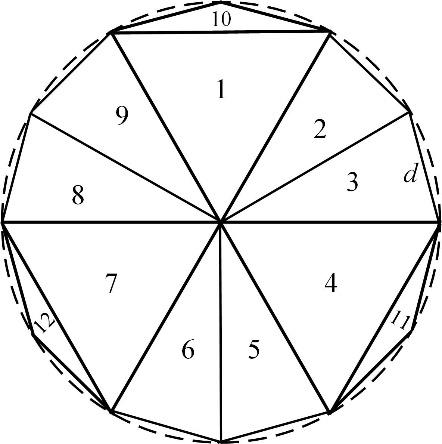
\includegraphics[width=0.4\columnwidth]{figs/fig2.jpg}
    \caption{Note: The figure shown is representative.}
    \label{fig2}
\end{figure}
\begin{enumerate}
\item 3; 4
\item 4; 3
\item 3; 3
\item 4; 4
\end{enumerate}

\item If a real variable x satisfies $3^{x^2} = 27 \times 9^x$, then the value of $\frac{2^{x^2}}{(2^x)^2}$ is:
\hfill{\brak{GATE~ES~2025}}
\begin{enumerate}
\item $2^{-1}$
\item $2^0$
\item $2^3$
\item $2^{1.5}$
\end{enumerate}

\item The number of patients per shift (X) consulting Dr. Gita in her past 100 shifts is shown in \figref{fig3}. If the amount she earns is \rupee$1000(X-0.2)$, what is the average amount (in \rupee) she has earned per shift in the past 100 shifts?
\hfill{\brak{GATE~ES~2025}}
\begin{figure}[H]
    \centering
    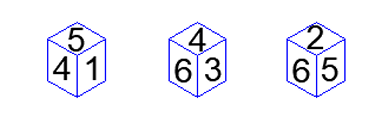
\includegraphics[width=0.6\columnwidth]{figs/fig3.png}
    \caption{Note: The figure shown is representative.}
    \label{fig3}
\end{figure}
\begin{enumerate}
\item 6,100
\item 6,300
\item 6,500
\item 6,700
\end{enumerate}
\end{enumerate}

\section*{Environmental Science and Engineering (ES)}

\subsection*{Q.11 -- Q.35 Carry ONE mark Each}

\begin{enumerate}[resume]
\item Assuming $s > |a|$; Laplace transform of $f(x) = \cosh ax$ is
\hfill{\brak{GATE~ES~2025}}
\begin{enumerate}
\item $\frac{s}{s^2+a^2}$
\item $\frac{a}{s^2+a^2}$
\item $\frac{s}{s^2-a^2}$
\item $\frac{a}{s^2-a^2}$
\end{enumerate}

\item For the ordinary differential equation $\frac{d^2y}{dx^2} + 4y = 0$, the general solution is
\hfill{\brak{GATE~ES~2025}}
\begin{enumerate}
\item $y = c_1 \cos 2x + c_2 \sin 2x$
\item $y = c_1 \cosh 2x + c_2 \sinh 2x$
\item $y = c_1 e^{2x} + c_2 e^{-2x}$
\item $y = c_1 e^{2x} \cos 2x + c_2 e^{-2x} \sin 2x$
\end{enumerate}

\item Consider the following two series \\
P: $\sum_{n=1}^{\infty} \frac{1}{n}$ \\
Q: $\sum_{n=1}^{\infty} \frac{1}{n^2}$ \\
Choose the correct option from the following
\hfill{\brak{GATE~ES~2025}}
\begin{enumerate}
\item P is convergent series; Q is divergent series
\item P is divergent series; Q is convergent series
\item Both P and Q are convergent series
\item Both P and Q are divergent series
\end{enumerate}

\item Choose the redox reaction from the following
\hfill{\brak{GATE~ES~2025}}
\begin{enumerate}
\item $H_2CO_3 \rightleftharpoons H^+ + HCO_3^-$
\item $Hg^{2+} + 2OH^- \rightleftharpoons Hg(OH)_2$
\item $C_6H_{12}O_6 + 6O_2 \rightleftharpoons 6CO_2 + 6H_2O$
\item $CaCO_3 (s) \rightleftharpoons Ca^{2+} + CO_3^{2-}$
\end{enumerate}

\item Which one of the following is performed by autotrophic bacteria?
\hfill{\brak{GATE~ES~2025}}
\begin{enumerate}
\item Aerobic biodegradation of organic matter
\item Anaerobic biodegradation of organic matter
\item Aerobic nitrification
\item Anaerobic de-nitrification
\end{enumerate}

\item For flood routing, consider the following statements \\
P: Hydrologic routing method uses continuity equation and momentum equation \\
Q: Hydraulic routing method uses continuity equation and energy equation \\
Choose the correct option from the following
\hfill{\brak{GATE~ES~2025}}
\begin{enumerate}
\item P is TRUE; Q is TRUE
\item P is TRUE; Q is FALSE
\item P is FALSE; Q is TRUE
\item P is FALSE; Q is FALSE
\end{enumerate}

\item For a gradually varied flow, consider the following statements \\
P: $y_n > y_c > y$ in M3 surface profile \\
Q: $y_n < y_c < y$ in S1 surface profile \\
where, $y_n$ is normal depth, $y_c$ is critical depth, and $y$ is flow depth. \\
Choose the correct option from the following
\hfill{\brak{GATE~ES~2025}}
\begin{enumerate}
\item P is TRUE; Q is TRUE
\item P is TRUE; Q is FALSE
\item P is FALSE; Q is TRUE
\item P is FALSE; Q is FALSE
\end{enumerate}

\item Match the following and choose the correct option from the following
\hfill{\brak{GATE~ES~2025}}
\begin{table}[H]
\centering
\begin{tabular}{ll}
\textbf{Type of reactor} & \textbf{Diagram} \\
1. Plug flow reactor & x. 
\includegraphics[height=1.5cm]{figs/fig4.jpg} \\
2. Continuously stirred tank reactor & y. 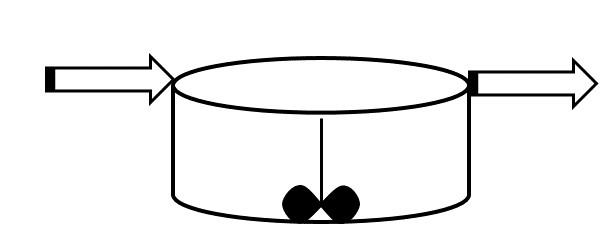
\includegraphics[height=1.5cm]{figs/fig5.jpg} \\
3. Batch reactor & z. 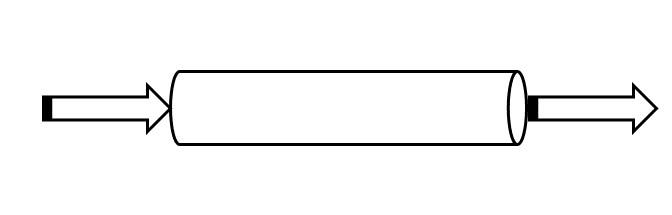
\includegraphics[height=1.5cm]{figs/fig6.jpg} \\
\multicolumn{2}{l}{
\includegraphics[height=0.75cm]{figs/fig4.jpg} indicates stirrer for mixing (not to scale)}
\end{tabular}
\end{table}
\begin{enumerate}
\item 1-x, 2-y, 3-z
\item 1-z, 2-y, 3-x
\item 1-y, 2-z, 3-x
\item 1-x, 2-z, 3-y
\end{enumerate}

\item Multiple effect evaporator is commonly used, in the zero liquid discharge (ZLD) scheme, for \_\_\_\_\_\_\_\_\_\_
\hfill{\brak{GATE~ES~2025}}
\begin{enumerate}
\item oxidation of organic pollutants
\item precipitation of heavy metals
\item concentrating reverse osmosis (RO) reject salts
\item performing selective ion exchange
\end{enumerate}

\item Consider the following statements \\
P: According to the National Ambient Air Quality Standards (Central Pollution Control Board, Govt. of India, notification 2009), annual time weighted average PM10 standard is more than PM2.5 standard. \\
Q: According to the National Air Quality Index released by Govt. of India in 2015, sub index value of PM10 can be less than that of PM2.5. \\
Choose the correct option from the following
\hfill{\brak{GATE~ES~2025}}
\begin{enumerate}
\item P is TRUE; Q is FALSE
\item P is FALSE; Q is TRUE
\item P is TRUE; Q is TRUE
\item P is FALSE; Q is FALSE
\end{enumerate}

\item Which option gives the components that are most likely to be present in the segregated combustible fraction (SCF) separated from raw mixed municipal solid waste (MSW)?
\hfill{\brak{GATE~ES~2025}}
\begin{enumerate}
\item plastics, paper, rubber, metals
\item plastics, paper, leather, glass
\item plastics, leather, textiles, rubber
\item plastics, rubber, textiles, food waste
\end{enumerate}

\item Correctly match the sustainable development goal (SDG) with its theme
\hfill{\brak{GATE~ES~2025}}
\begin{table}[H]
\centering
\begin{tabular}{ll}
\textbf{SDG} & \textbf{Theme} \\
i. SDG 6 & p. Good Health and Well-being \\
ii. SDG 11 & q. Responsible Consumption and Production \\
iii. SDG 3 & r. Sustainable Cities and Communities \\
iv. SDG 12 & s. Clean Water and Sanitation
\end{tabular}
\end{table}
\begin{enumerate}
\item i-q, ii-r, iii-p, iv-s
\item i-s, ii-r, iii-p, iv-q
\item i-s, ii-r, iii-q, iv-p
\item i-p, ii-q, iii-r, iv-s
\end{enumerate}

\item Choose the correct option regarding the Basel Convention
\hfill{\brak{GATE~ES~2025}}
\begin{enumerate}
\item Almost all the nations of the world assembled for the first time in the history to discuss and find out the solution for a common environmental problem.
\item It was for formulating the strategies and guidelines to reduce CO2 and CH4 emissions to control the global warming.
\item It was for formulating the strategies and guidelines to control the release of acidic gases that can cause acid rains in another country.
\item It was for formulating the strategies and guidelines for the trans-boundary movement of hazardous wastes.
\end{enumerate}

\item Consider the following statements \\
(i) Environmental pollutant concentration is generally modeled using lognormal distribution. \\
(ii) Environmental pollutant concentration is generally modeled using Poisson distribution. \\
(iii) The weekly rate of exceedance of environmental pollutant concentration with regards to a given standard is generally modeled using lognormal distribution. \\
(iv) The weekly rate of exceedance of environmental pollutant concentration with regards to a given standard is generally modeled using Poisson distribution. \\
Choose the correct option(s) from the following
\hfill{\brak{GATE~ES~2025}}
\begin{enumerate}
\item (i) and (iv) are correct
\item (i) is correct and (iii) is incorrect
\item (ii) and (iv) are correct
\item (ii) and (iv) are incorrect
\end{enumerate}

\item Choose the correct statement(s) from the following regarding the structure/reproduction of microorganisms
\hfill{\brak{GATE~ES~2025}}
\begin{enumerate}
\item Prokaryotes do not have nucleus but Eukaryotes have nucleus.
\item Both Prokaryotes and Eukaryotes have nucleus.
\item No binary fission happens in Eukaryotes, however, Prokaryotes rely on binary fission for reproduction.
\item Both Prokaryotes and Eukaryotes rely on binary fission for reproduction.
\end{enumerate}

\item Consider the following statements related to nitrification process: \\
(i) Electron acceptor type vary depending on whether nitrosomonas or nitrobacter is involved. \\
(ii) Predominant carbon source is organic matter. \\
(iii) Predominant carbon source is inorganic carbon. \\
(iv) Electron donor during conversion of ammonium ions to nitrite ions is ammonium ions. \\
Choose the correct option(s) from the following
\hfill{\brak{GATE~ES~2025}}
\begin{enumerate}
\item (iii) and (iv) are correct
\item (i) and (ii) are correct
\item (i) is incorrect and (iii) is correct
\item (ii) is correct and (iii) is incorrect
\end{enumerate}

\item Stubble burning results in release of particulate matter, volatile organic compounds, oxides of nitrogen and sulfur, to name a few. A researcher is planning to use a conventional Gaussian dispersion model to estimate the contribution of stubble burning in a nearby state to air pollution in New Delhi. Choose the option(s) which could explain the possible limitations in this approach
\hfill{\brak{GATE~ES~2025}}
\begin{enumerate}
\item assumption of steady state conditions e.g. constant wind speed, wind direction, and emission, etc. in conventional Gaussian dispersion models
\item non-accounting of wet and dry deposition in conventional Gaussian dispersion models
\item non-handling of chemical transformation of pollutants in conventional Gaussian dispersion models
\item requirement of more computational resources by conventional Gaussian dispersion models compared to chemical transport models
\end{enumerate}

\item Choose the correct option(s) from the following in the plastic waste management
\hfill{\brak{GATE~ES~2025}}
\begin{enumerate}
\item Plastic wastes may be burnt to generate fuel oil and fuel gas.
\item Plastic wastes along with bitumen may be used for road/pavement construction.
\item Polyethylene terephthalate (PET) and high density polyethylene (HDPE) are the most common plastics for recycling.
\item Plastics made of branched monomers can be easily recycled.
\end{enumerate}

\item Choose the option(s) giving the correct process flow-sheet for producing refuse derived fuel (RDF) from the segregated waste collected in the dry waste containers (blue coloured containers of the municipal solid waste (MSW) collection scheme).
\hfill{\brak{GATE~ES~2025}}
\begin{enumerate}
\item 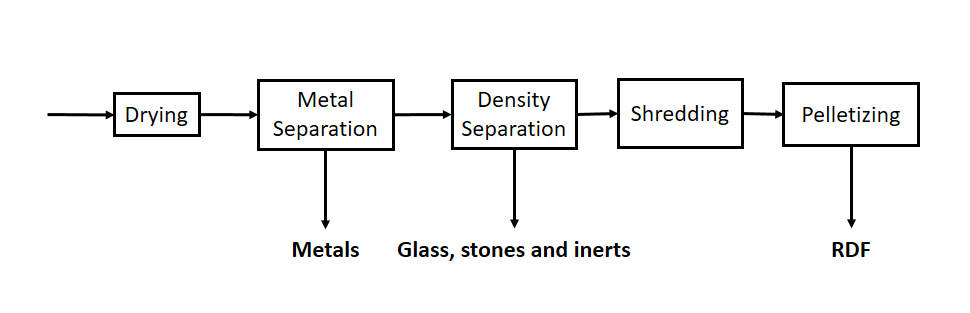
\includegraphics[width=\columnwidth]{figs/fig7.png}
\item 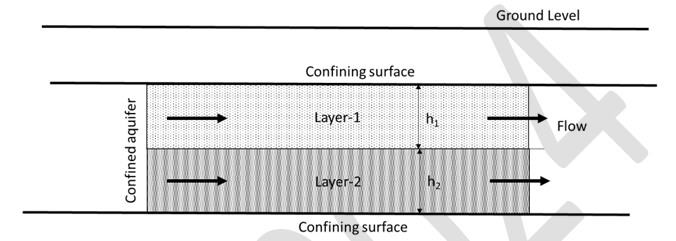
\includegraphics[width=\columnwidth]{figs/fig8.png}
\item 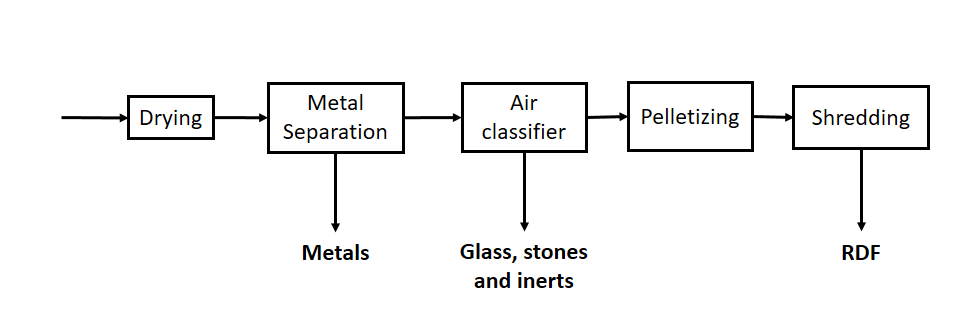
\includegraphics[width=\columnwidth]{figs/fig9.png}
\item 
\includegraphics[width=\columnwidth]{figs/fig10.png}
\end{enumerate}

\item Choose the correct option(s) from the following regarding the symbiotic relationships
\hfill{\brak{GATE~ES~2025}}
\begin{enumerate}
\item Lichens are a symbiotic association of fungi and bacteria. They can survive in extreme conditions of air pollution.
\item Lichens are a symbiotic association of fungi and bacteria. The fungi can absorb water and minerals from atmosphere, and bacteria can generate foods.
\item Lichens are a symbiotic association of fungi and algae. They can survive in extreme conditions, but are very sensitive to air pollution.
\item Lichens are a symbiotic association of fungi and algae. The fungi can absorb water and minerals from atmosphere, and algae can generate food through photosynthesis.
\end{enumerate}

\item Methane hydrates have special crystal structure of water, where methane gas molecules are trapped. Choose the correct option(s) from the following
\hfill{\brak{GATE~ES~2025}}
\begin{enumerate}
\item Methane hydrates exist in abundance near the ocean bed, where the pressure is high enough for their existence.
\item Methane hydrates exist in abundance in the polar regions, where the temperature is low enough for their existence.
\item Methane hydrates can be a huge source of energy, but can accelerate global warming considerably if the entrapped methane is released to the atmosphere.
\item Methane hydrates can be a huge source of energy, but difficult to exploit commercially.
\end{enumerate}

\item Choose the correct option(s) from the following regarding urban environment
\hfill{\brak{GATE~ES~2025}}
\begin{enumerate}
\item Urban heat island can exacerbate urban flooding by intensifying rainfall intensity.
\item Urban canyons increase ventilation by trapping heat and thus enhancing urban heat island effect.
\item Program evaluation and review technique (PERT) is always used to estimate the economic impact of mitigation strategies for urban heat island effect.
\item In general, land surfaces in urban areas emit more long wave radiation compared to those in rural areas, and thus contribute to higher night time temperature.
\end{enumerate}

\item Choose the correct option(s) from the following regarding cumulative toxicity
\hfill{\brak{GATE~ES~2025}}
\begin{enumerate}
\item Bioaccumulation is the process by which a living organism keeps on accumulating pollutants in its body due to continuous exposure, whereas, bio-magnification is the process by which higher order organisms accumulate more pollutants than the lower order organisms in a food chain.
\item Biomagnification is the process by which a living organism keeps on accumulating pollutants in its body due to continuous exposure, whereas, bioaccumulation is the process by which higher order organisms accumulate more pollutants than the lower order organisms in a food chain.
\item Bioaccumulation and biomagnification are possible with heavy metals, but not with pesticides and pharmaceutical compounds.
\item Bioaccumulation and biomagnification are possible with heavy metals, pesticides and pharmaceutical compounds.
\end{enumerate}

\item $\lim_{x\to0} \left( \frac{\ln(1+x)^2}{\sin x} \right)$ is \_\_\_\_\_\_\_\_\_\_\_\_\_\_ \textit{(rounded off to two decimal places)}.
\hfill{\brak{GATE~ES~2025}}

\item An unconfined aquifer of areal extent 20 $km$ $\times$ 20 $km$ has hydraulic conductivity of 4 $m/day$, porosity of 0.32, and storage coefficient (specific yield) of 0.18. If the initial saturated thickness of the aquifer is 30 $m$, and $4 \times 10^8$ $m^3$ of water is extracted from the aquifer, then the decline in the saturated thickness is \_\_\_\_\_\_\_\_\_\_\_\_\_\_ $m$. \textit{(rounded off to two decimal places)}
\hfill{\brak{GATE~ES~2025}}

\subsection*{Q.36 -- Q.65 Carry TWO marks Each}

\item A researcher added certain amount of $HgCl_2$ to water at pH 10. He calculated the expected concentration of mercury in the water. He asked his student to measure the concentration. His student used an instrument that can measure only the free metal, $Hg^{2+}$. The student observed that the concentration measured by him was significantly less than the concentration calculated by the researcher. How can he explain the paradox to the researcher? \\
Explanation 1: Significant fraction of the mercury would have changed phase from aqueous to gaseous phase, thus leaving less mercury in the water \\
Explanation 2: Fraction of the mercury added to water would have formed aqueous complexes \\
Explanation 3: Fraction of the mercury added to water could have precipitated \\
Choose the correct option from the following
\hfill{\brak{GATE~ES~2025}}
\begin{enumerate}
\item only Explanation 1 is correct
\item Explanations 1 and 2 are correct
\item Explanations 1 and 3 are correct
\item Explanations 2 and 3 are correct
\end{enumerate}

\item Correctly label the speciation diagram below:
\hfill{\brak{GATE~ES~2025}}
\begin{figure}[H]
    \centering
    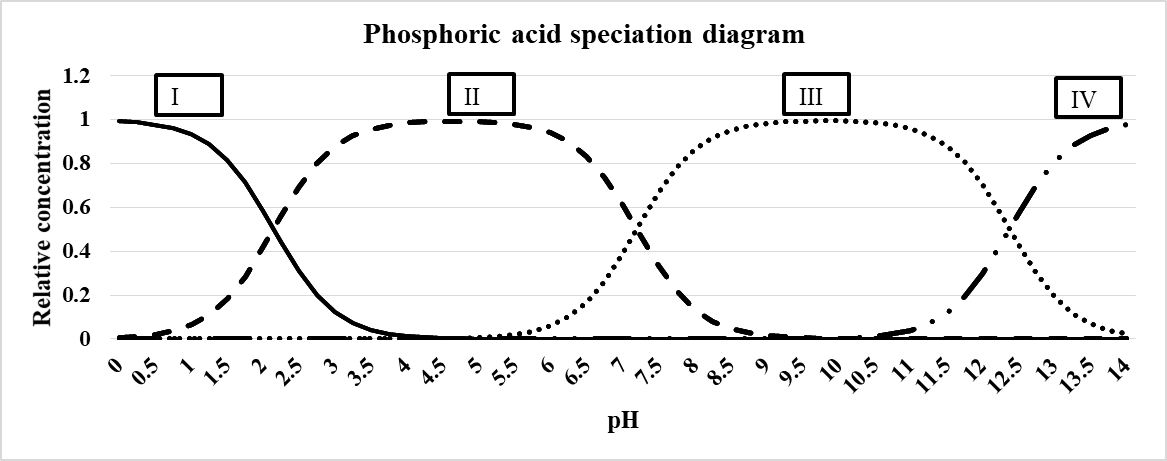
\includegraphics[width=\columnwidth]{figs/fig11.png}
    \label{fig11}
\end{figure}
\begin{enumerate}
\item I= $PO_4^{3-}$, II= $HPO_4^{2-}$, III= $H_2PO_4^-$, IV= $H_3PO_4$
\item I= $H_3PO_4$, II= $HPO_4^{2-}$, III= $H_2PO_4^-$, IV= $PO_4^{3-}$
\item I= $H_3PO_4$, II= $H_2PO_4^-$, III= $HPO_4^{2-}$, IV= $PO_4^{3-}$
\item I= $PO_4^{3-}$, II= $H_2PO_4^-$, III= $H_3PO_4$, IV= $HPO_4^{2-}$
\end{enumerate}

\item Consider the following statements on microbial metabolism \\
(i) Utilization of carbon for cell synthesis is termed as anabolism. \\
(ii) During catabolism, adenosine triphosphate (ATP) is converted into adenosine diphosphate (ADP). \\
Choose the correct option from the following
\hfill{\brak{GATE~ES~2025}}
\begin{enumerate}
\item (i) and (ii) are correct
\item (i) and (ii) are incorrect
\item (i) is correct and (ii) is incorrect
\item (i) is incorrect and (ii) is correct
\end{enumerate}

\item Consider the following figure of an activated sludge process (ASP), depicting the flow (\textbf{Q}), substrate (\textbf{S}), and microorganism concentration (\textbf{X}) at various points in the system, where subscripts ``\textbf{0}'', ``\textbf{r}'', ``\textbf{w}'', ``\textbf{e}'', and ``\textbf{i}'' indicate influent, recycle line, wastage, effluent, and flow from aeration tank to settling tank, respectively. Note that influent to the ASP has microbes too. \textbf{V} is volume of aeration tank. Choose the correct option for net rate of formation of microorganisms in the system at steady state, from the following
\hfill{\brak{GATE~ES~2025}}
\begin{figure}[H]
    \centering
    
\includegraphics[width=\columnwidth]{figs/fig12.png}
    \caption{ASP Diagram}
    \label{fig12}
\end{figure}
\begin{enumerate}
\item $\frac{(Q-Q_w)X_e + Q_wX_r - QX_0}{V}$
\item $\frac{(Q-Q_w)X_e + Q_wX_r}{V}$
\item $\frac{(Q-Q_w)X_e + Q_wX_r}{VX}$
\item $\frac{(Q+Q_r)X_i + Q_wX_r}{VX}$
\end{enumerate}

\item Consider the following statements \\
(i) Sound pressure changes with distance from the source \\
(ii) Sound power is a property of the source \\
(iii) Sound intensity is sound power per unit volume \\
Choose the correct option from the following
\hfill{\brak{GATE~ES~2025}}
\begin{enumerate}
\item (i), (ii), and (iii) are correct
\item only (i) and (ii) are correct
\item only (i) and (iii) are correct
\item only (ii) and (iii) are correct
\end{enumerate}

\item At a pressure of 1 atmosphere and temperature of $25\celsius$, 365 $\mu g m^{-3}$ of a pollutant corresponds to mixing ratio of 139 parts per billion (ppb). The atomic weights: $C$ - 12, $H$ - 1, $O$ - 16, $N$ - 14 and $S$ - 32. Which one of the following options most closely represents the pollutant
\hfill{\brak{GATE~ES~2025}}
\begin{enumerate}
\item $SO_2$
\item $NO_2$
\item $O_3$
\item $CO$
\end{enumerate}

\item Which option gives the best control strategies for Dioxins and Furans in the flue gas emitted from waste incineration facilities?
\hfill{\brak{GATE~ES~2025}}
\begin{enumerate}
\item Avoid burning polystyrene (PS) and polyethylene (PE); ensure the furnace temperature above 1000 $\celsius$; and use a bag filter for cleaning the flue gas.
\item Avoid burning polyvinyl chloride (PVC); quickly cool down the flue gas through the temperature range 400 - 250 $\celsius$; and use an activated carbon treatment for the flue gas.
\item Avoid burning food wastes; ensure the furnace temperature above 900 $\pm$ 50 $\celsius$; and use an electrostatic precipitator (ESP) for cleaning the flue gas.
\item Avoid burning metal bearing waste; ensure the flue gas temperature above 1000 $\celsius$; and use a venturi scrubber for cleaning the flue gas.
\end{enumerate}

\item Choose the correct option(s) from the following regarding the solubility in water
\hfill{\brak{GATE~ES~2025}}
\begin{enumerate}
\item Water is a polar molecule because of the asymmetric distribution of charge between the oxygen and hydrogen atoms of the water molecule.
\item In a water molecule, the electrons shared between oxygen and hydrogen are attracted more towards the hydrogen atom.
\item Non-polar compounds are highly soluble in water because of their strong interaction with water molecules.
\item Aromaticity and charge of molecules influence their solubility in water.
\end{enumerate}

\item If microbial growth occurs under substrate unlimited conditions, according to Monod's kinetics, choose the correct option(s) from the following
\hfill{\brak{GATE~ES~2025}}
\begin{enumerate}
\item Microbial growth follows zero order with respect to substrate concentration.
\item Microbial growth follows first order with respect to substrate concentration.
\item Specific growth rate is half of maximum specific growth rate.
\item Specific growth rate is almost equal to maximum specific growth rate.
\end{enumerate}

\item Choose the correct option(s) for removing solids from water.
\hfill{\brak{GATE~ES~2025}}
\begin{enumerate}
\item chlorination
\item coagulation-flocculation-sedimentation followed by slow sand filtration
\item chlorination followed by aeration
\item slow sand filtration
\end{enumerate}

\item According to the Bio-Medical Waste Management Rules, 2016, choose the correct option(s) from the following
\hfill{\brak{GATE~ES~2025}}
\begin{enumerate}
\item Bio-medical waste generated should be taken to a common bio-medical waste management facility except for rural areas where common facility is not available.
\item Bio-medical waste generated should not be taken out of the hospital premise as it may contain dangerous pathogenic organisms.
\item The red bag containing the human anatomical wastes like amputated body parts, cotton and bandages contaminated with body fluids, etc. should be treated using autoclave or hydroclave to kill the pathogenic organisms.
\item Increasing operational temperature of an autoclave from 121 $\celsius$ (pressure 15 psi) to 149 $\celsius$ (pressure 52 psi), the residence time requirement for treating bio-medical waste will be reduced by 15 minutes.
\end{enumerate}

\item A residential family is considering two cities for relocation. The data related to pollutant exposure and associated health cost per year are given in \figref{fig13}. The pollutant exposure is characterized in high, mild and low exposure categories with respective probability values. The difference in expected value of health cost of City 1 with respect to that of City 2 is \_\_\_\_\_\_\_\_\_\_\_\_\_\_ lakhs/year. \textit{(rounded off to two decimal places)}.
\hfill{\brak{GATE~ES~2025}}
\begin{figure}[H]
    \centering
    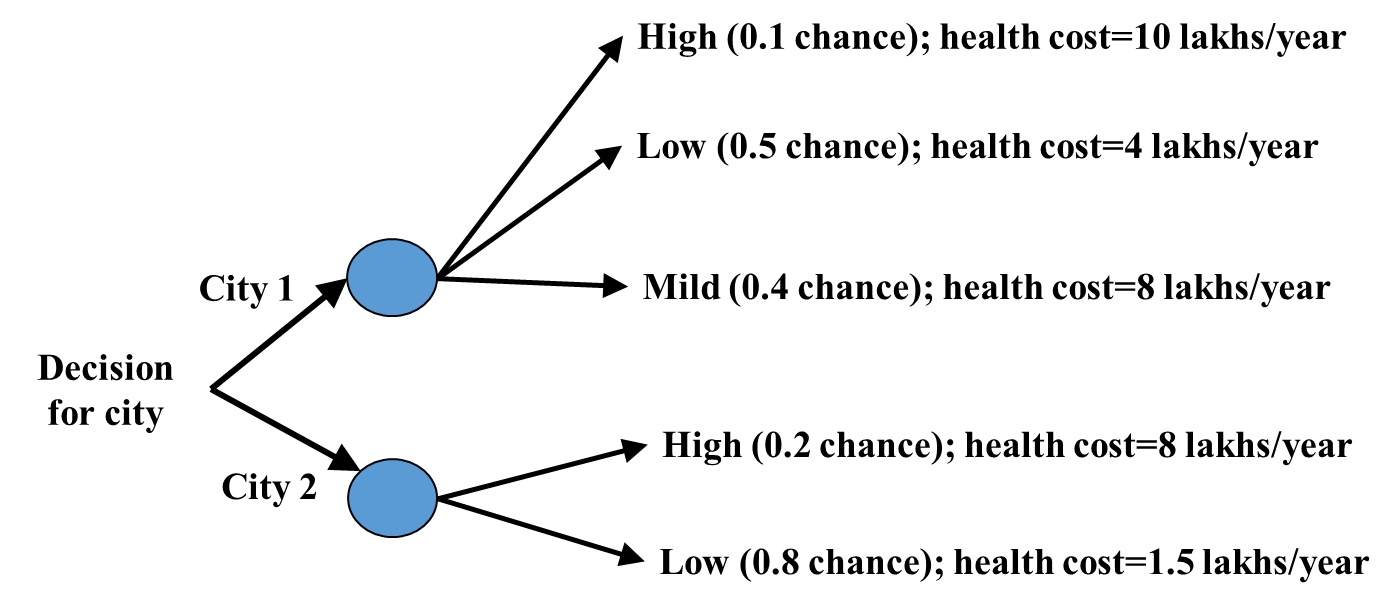
\includegraphics[width=0.8\columnwidth]{figs/fig13.png}
    \caption{Figure for Q.47}
    \label{fig13}
\end{figure}

\item The following is a system of linear equations
\begin{align*}
x - 2y + z = 34 \\
2x + y + z = 102 \\
x + y - 3z = 17 
\end{align*}
The value of $(x + y + z)$ is \_\_\_\_\_\_\_\_\_\_\_\_\_\_. \textit{(rounded off to two decimal places)} \hfill{\brak{GATE~ES~2025}}

\item The value of $\int_0^\infty \frac{\sin 4x}{\pi x} dx$ is \_\_\_\_\_\_\_\_\_\_\_\_\_\_. \textit{(rounded off to two decimal places)}
\hfill{\brak{GATE~ES~2025}}

\item A tank has inflow, outflow and stirring mechanism. Initially, the tank holds 500 $L$ of a brine solution of concentration 200 $g/L$. At t = 0, an inflow of another brine solution of concentration 100 $g/L$ starts entering the tank at the rate of 15 $L/minute$. At the same time the outflow of thoroughly stirred mixture also takes place at the same rate so that the volume of brine in the tank remains constant. The brine concentration $C$ ($g/L$) in the tank at any time $t$ (minute) can be expressed by the following differential equation 
\begin{align*}
\frac{dC}{dt} + 0.03 C = 3
\end{align*}
The brine concentration in the tank at $t$ = 1.5 hour is \_\_\_\_\_\_\_\_\_\_\_\_\_\_ $g/L$. \textit{(rounded off to two decimal places)}
\hfill{\brak{GATE~ES~2025}}

\item Aerobic biomass has yield coefficient value of 0.4 for glucose (molecular weight = 180 $g/mole$) substrate. Bacteria is represented as $C_5H_7O_2N$ (molecular weight = 113 $g/mole$). Assume that no endogenous metabolism occurs. The percentage of carbon going into $CO_2$ from 1 $mole/L$ glucose is \_\_\_\_\_\_\_\_\_\_\_\_\_\_. \textit{(rounded off to two decimal places)} \hfill{\brak{GATE~ES~2025}}

\item The following figure (not to scale) depicts a rainfall hyetograph for a storm over a catchment. If the storm produced a direct runoff of 12.5 $mm$, then the $\phi$-index of the storm for the catchment is \_\_\_\_\_\_\_\_\_\_\_\_\_\_ $mm/hour$. \textit{(rounded off to two decimal places)} \hfill{\brak{GATE~ES~2025}}
\begin{figure}[H]
    \centering
    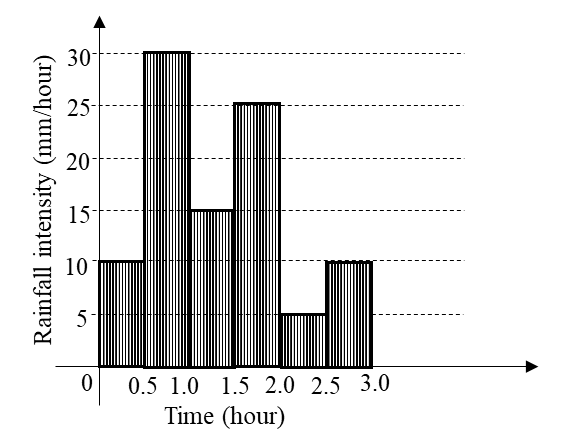
\includegraphics[width=0.6\columnwidth]{figs/fig14.png}
    \caption*{Figure for Q.52}
\end{figure}

\item The following table and figure (not to scale) show characteristics of a catchment. \hfill{\brak{GATE~ES~2025}}

\begin{table}[H]
\centering
\begin{tabular}{|l|c|c|c|}
\hline
\textbf{Sub catchment} & \textbf{Area (ha)} & \textbf{Runoff coefficient} & \textbf{Time of concentration} \\
\hline
P & 750 & 0.5 & 1 hour \\
Q & 1000 & 0.6 & 2 hour \\
R & 1500 & 0.6 & 3 hour \\
S & 2000 & 0.7 & 4 hour \\
\hline
\end{tabular}
\end{table}
\begin{figure}[H]
    \centering
    
\includegraphics[width=0.45\columnwidth]{figs/fig15.png}
\end{figure}
The hyetograph resulting from a storm that occurred uniformly over the catchment, is as follows:
\begin{figure}[H]
    \centering
    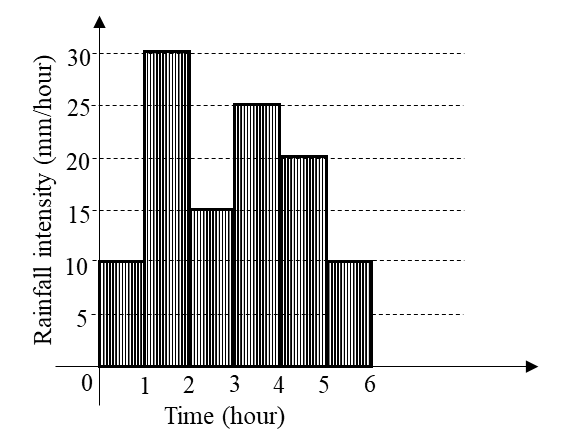
\includegraphics[width=0.45\columnwidth]{figs/fig16.png}
\end{figure}
Assuming a constant base flow of $40 m^3/s$, the peak of the runoff hydrograph produced by storm for the catchment at the outlet $\textbf{\textit{O}}$ is \_\_\_\_\_\_\_\_\_\_\_\_\_\_ $m^3/s$. \textit{(rounded off to two decimal places)}

\item A homogeneous isotropic confined aquifer of uniform thickness 30 m has hydraulic conductivity of 5 m/day and porosity of 0.3. There are two observation wells $X$ and $Y$ along a radial line from a fully penetrating pumping well at 100 m and 200 m distance, respectively. The well is pumped at a uniform rate to produce steady drawdown of 5 m at $X$ and 3 m at $Y$. If a non-reactive pollutant enters at the observation well $Y$, then the time taken by the pollutant (under advection) to reach the observation well $X$ is \_\_\_\_\_\_\_\_\_\_\_\_\_\_ days. \textit{(rounded off to two decimal places)} \hfill{\brak{GATE~ES~2025}}

\item A pipe line $O$ $P$ $Q$ $R$ branches into three pipes $X$, $Y$, and $Z$ between points $P$ and $Q$ as shown in figure (not to scale). Diameter ($d$) and length ($l$) of each pipe are as presented in figure and all pipes are of same material having friction factor ($f$) of 0.02. Assume acceleration due to gravity ($g$) as 10.0 $m/s^2$. If the head difference between $P$ and $Q$ is 10 m, then the head loss between $Q$ and $R$ is \_\_\_\_\_\_\_\_\_\_\_\_\_\_ m. \textit{(rounded off to two decimal places)}
\hfill{\brak{GATE~ES~2025}}
\begin{figure}[H]
    \centering
    
\includegraphics[width=0.8\columnwidth]{figs/fig17.png}
    \caption*{Figure for Q.55}
\end{figure}

\item A circular sewer pipe, having Manning's coefficient ($n$) of 0.01, is laid at a bed slope of 1:100. If it is flowing 80\% full for a discharge of $2 m^3/s$, then its diameter is \_\_\_\_\_\_\_\_\_\_\_\_\_\_ m. \textit{(rounded off to three decimal places)} \hfill{\brak{GATE~ES~2025}}

\item You conducted a batch experiment in the lab for 10 minutes to degrade a toxic compound, which follows first order kinetics. The compound degrades from $2 \times 10^{-3}$ M to $2 \times 10^{-4}$ M. The information from the lab experiment will be used to design a plug flow reactor in field conditions. Given field conditions:
\begin{itemize}
    \item Flow rate of contaminated water to be treated: 1 $m^3$/hour
    \item Concentration of toxic compound in contaminated water: $5 \times 10^{-1} M$
    \item Target concentration of toxic compound in treated water: $1 \times 10^{-4} M$
    \item Temperature is same in lab and field conditions.
\end{itemize}
The required volume of the plug flow reactor is \_\_\_\_\_\_\_\_\_\_\_\_\_\_ $m^3$. \textit{(rounded off to two decimal places)} \hfill{\brak{GATE~ES~2025}}

\item A common effluent treatment plant with a capacity of 2 million litres per day (MLD) employs reverse osmosis (RO) for water reuse. The RO unit removes 95\% of the total dissolved solids (TDS) and the water recovery rate is 70\%. If the TDS concentration in the RO feed is 8000 parts per million (ppm), the TDS in the RO reject is \_\_\_\_\_\_\_\_\_\_\_\_\_\_ g/L. \textit{(rounded off to one decimal place)} \hfill{\brak{GATE~ES~2025}}

\item A boiler burns coal at a rate of 1 kg/s. If the coal has 3\% sulfur content, assuming that there is no sulfur in ash, SO$_2$ emitted is \_\_\_\_\_\_\_\_\_\_\_\_\_\_ kg/day. \textit{(rounded off to nearest integer)}
\hfill{\brak{GATE~ES~2025}}

\item A particle dispersoid has 1510 spherical particles of uniform density. An air purifier is proposed to be used to remove these particles. The diameter specific number of particles in the dispersoid, along with the number removal efficiency of the proposed purifier is shown in the following table: \hfill{\brak{GATE~ES~2025}}
\begin{table}[H]
\centering
\begin{tabular}{|c|c|c|}
\hline
\textbf{Diameter of the} & \textbf{Number of particles} & \textbf{Number removal} \\
\textbf{particle ($\mu$m)} & & \textbf{efficiency (\%)} \\
\hline
1 & 1000 & 99 \\
10 & 500 & 75 \\
100 & 10 & 10 \\
\hline
\end{tabular}
\end{table}
The overall mass removal efficiency of the proposed purifier is \_\_\_\_\_\_\_\_\_\_\_\_\_\_ \%. \textit{(rounded off to one decimal place)}

\item An incandescent light bulb operated for two hours per day uses 12.2 $kWh$ of energy per month. Burning of one kg of coal generates 2 $kWh$ of electrical energy and releases $7 g$ of PM10. The reduction in PM10 emitted per month, if this incandescent bulb is replaced with a light emitting diode (LED) bulb which consumes 1/6th of energy, is \_\_\_\_\_\_\_\_\_\_\_\_\_\_ $g$. \textit{(rounded off to one decimal place)} \hfill{\brak{GATE~ES~2025}}

\item A street sweeping machine starts from point $P$ and ends at $S$, as shown in the network of streets below. It sweeps all the streets at least once. \hfill{\brak{GATE~ES~2025}}
\begin{figure}[H]
    \centering
    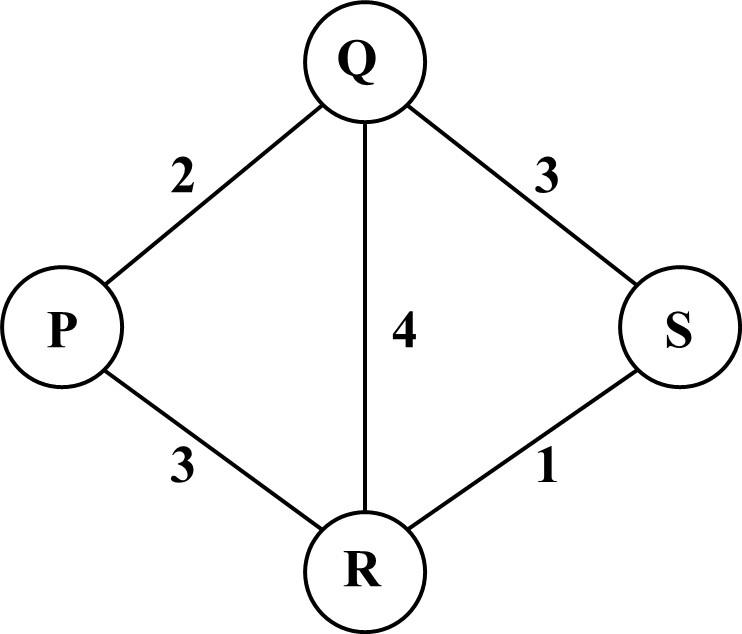
\includegraphics[width=0.5\columnwidth]{figs/fig18.jpg}
\end{figure}
Length of the streets, in $km$, are shown on the network. The minimum distance travelled by the sweeping machine for completing the job of sweeping all the streets is \_\_\_\_\_\_\_\_\_\_\_\_\_\_ $km$. \textit{(rounded off to nearest integer)}

\item A solid waste of composition $C_{60}H_{135}O_{50}N_5$ is to be composted aerobically in a closed vessel mechanical composting facility. Given: all ammonia generated escapes the facility; air contains 23\% of Oxygen by weight; 100\% excess air requirement for the closed vessel composting facility. The atomic weights: $C$ - 12, $H$ - 1, $O$ - 16, $N$ - 14. The actual air required for composting is \_\_\_\_\_\_\_\_\_\_\_\_\_\_ $kg$ per $kg$ waste. \textit{(rounded off to one decimal place)} \hfill{\brak{GATE~ES~2025}}

\item An industry releases three greenhouse gases (GHGs), $CO_2$ (5 $kg/day$), $CH_4$ (0.5 $kg/day$), and $N_2O$ (0.1 $kg/day$). The industry flares the $CH_4$ before it is released to the atmosphere. The Global Warming Potential (GWP) are as follows: $CO_2$ = 1, $CH_4$ = 21, $N_2O$ = 310. The annual GWP of GHGs released from the industry is \_\_\_\_\_\_\_\_\_\_\_\_\_\_ $kg$ $CO_2$ equivalent. \textit{(rounded off to the nearest integer)} \hfill{\brak{GATE~ES~2025}}

\item Water from a hand pump located near a landfill has 1 $mg/L$ arsenic (oral carcinogenic potency factor = 1.75 $(kg-day)/mg$). A person who lives nearby drinks 2 $L/day$ water from this hand pump for 10 years. Assume body weight of 70 $kg$ and 70 years as average life duration. Chances of this person getting excess risk of cancer is \_\_\_\_\_\_\_\_\_\_\_\_\_\_ $\times 10^{-3}$. \textit{(rounded off to three decimal places)} \hfill{\brak{GATE~ES~2025}}

\end{enumerate}

\bigskip
\begin{align*}
\textbf{END OF THE QUESTION PAPER}
\end{align*}

\end{document}
